\documentclass[12pt]{article}

\usepackage[margin=1in]{geometry}
\usepackage{amsmath}
\usepackage{amssymb}
\usepackage{graphicx}
\usepackage{booktabs}
\usepackage{hyperref}
\usepackage[capitalise]{cleveref}
\usepackage{microtype}
\usepackage{parskip}
\usepackage{xcolor}

\usepackage{tikz}
\usetikzlibrary{arrows.meta, positioning, shapes.geometric, calc, fit}

% Figures live in ./images (generated by code/gen_figures_integral.m)
\graphicspath{{./}}

% Draft review flag: \verify{note} renders an inline orange callout.
% Redefine to \newcommand{\verify}[1]{} to suppress all flags in a clean build.
\newcommand{\verify}[1]{\textcolor{orange}{\textbf{[?~#1]}}}

\newcommand{\figplaceholder}[2][3in]{%
  \begin{center}
  \fbox{\parbox{#1}{\centering\vspace{0.5in}\textit{[Figure: #2]}\vspace{0.5in}}}
  \end{center}
}

% Include a generated figure if it exists; otherwise show a placeholder.
\newcommand{\genfig}[2]{%
  \IfFileExists{#1}{\includegraphics[width=\linewidth]{#1}}%
                   {\figplaceholder[4in]{#2 --- run code/gen\_figures\_integral.m}}%
}

\hypersetup{
  pdftitle  = {USV Control Case Study, Part 2: Integral control},
  pdfauthor = {Brian Bingham},
}

\begin{document}

\begin{center}
   \setlength{\parskip}{0pt}
  {\LARGE USV Control Case Study\par}
  {\Large Part 2: Integral control\par}
  \vspace{0.8em}
  Brian Bingham \quad\textbar\quad Fall 2026
\end{center}

% ===========================================================================
\section{Why Proportional Control Leaves an Error}
\label{sec:why_error}
% ===========================================================================

Part 1 closed a proportional loop around the first-order surge model
\begin{equation}
  G_{v_x}(s) = \frac{K_{v_x}}{\tau_{v_x} s + 1}
  \label{eq:surge_plant}
\end{equation}
and found that a unit step in desired speed leaves a steady-state error
\begin{equation}
  e_{ss} = \frac{1}{1 + K_P K_{v_x}}.
  \label{eq:p_error}
\end{equation}

The error has a physical cause.  Holding a constant speed against hull drag takes a constant throttle.  At steady state the plant output is its DC gain times its input, $y_{ss} = K_{v_x} u_{ss}$, so holding $y_{ss}$ takes throttle $u_{ss} = y_{ss}/K_{v_x}$.  A proportional controller only produces throttle when there is error, $u = K_P e$, so the only way to keep supplying $u_{ss}$ is to keep an error of
\[
  e_{ss} = \frac{u_{ss}}{K_P} \neq 0.
\]
(Substituting $y_{ss} = 1 - e_{ss}$ and solving recovers \cref{eq:p_error}.)  The proportional controller needs the error to do its job.  Raising $K_P$ shrinks the error the controller needs, but it never removes it.

What we want is a controller term that can hold a nonzero throttle while the error is zero.

% ===========================================================================
\section{Adding an Integral Term}
\label{sec:pi}
% ===========================================================================

The proportional-integral (PI) control law adds a term proportional to the accumulated error:
\begin{equation}
  u(t) = \underbrace{K_P\, e(t)}_{u_P(t)} \;+\; \underbrace{K_I \int_0^t e(\tau)\,d\tau}_{u_I(t)}
  \qquad\Longleftrightarrow\qquad
  C(s) = K_P + \frac{K_I}{s} = \frac{K_P s + K_I}{s}.
  \label{eq:pi}
\end{equation}
In a block diagram, the two terms act in parallel on the error (\cref{fig:pi_block}).

\begin{figure}[htbp]
\centering
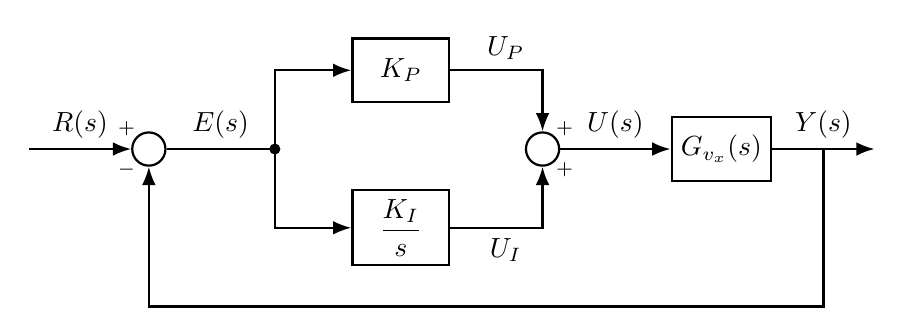
\begin{tikzpicture}[
  >=Latex, thick,
  block/.style = {draw, rectangle, minimum height=2.3em, minimum width=3.5em},
  sum/.style   = {draw, circle, inner sep=0pt, minimum size=1.2em},
]
  \node[coordinate]                    (rin)  {};
  \node[sum,   right=1.3cm of rin]     (esum) {};
  \coordinate                          (split) at ($(esum)+(1.6,0)$);
  \node[block] (KP) at ($(split)+(1.6, 1.0)$) {$K_P$};
  \node[block] (KI) at ($(split)+(1.6,-1.0)$) {$\dfrac{K_I}{s}$};
  \node[sum]   (usum) at ($(split)+(3.4,0)$) {};
  \node[block, right=1.4cm of usum]    (G)    {$G_{v_x}(s)$};
  \node[coordinate, right=1.3cm of G]  (yout) {};

  \node[font=\scriptsize, inner sep=0pt, anchor=south east] at (esum.north west) {$+$};
  \node[font=\scriptsize, inner sep=0pt, anchor=north east] at (esum.south west) {$-$};
  \node[font=\scriptsize, inner sep=0pt, anchor=south west] at (usum.north east) {$+$};
  \node[font=\scriptsize, inner sep=0pt, anchor=north west] at (usum.south east) {$+$};

  \draw[->] (rin)  -- node[above]{$R(s)$} (esum);
  \draw     (esum) -- node[above]{$E(s)$} (split);
  \fill (split) circle (2pt);
  \draw[->] (split) |- (KP.west);
  \draw[->] (split) |- (KI.west);
  \draw[->] (KP.east) -| node[above, pos=0.3]{$U_P$} (usum.north);
  \draw[->] (KI.east) -| node[below, pos=0.3]{$U_I$} (usum.south);
  \draw[->] (usum) -- node[above]{$U(s)$} (G);
  \draw[->] (G)    -- node[above]{$Y(s)$} (yout);

  \coordinate (fbk) at ($(G.east)!0.5!(yout)$);
  \draw[->] (fbk) -- ++(0,-2.0) -| (esum.south);
\end{tikzpicture}
\caption{PI control of USV speed.  The integral path $K_I/s$ runs in parallel with the proportional gain.}
\label{fig:pi_block}
\end{figure}

\subsection{The Integrator Accumulates Error}

The integral term is easiest to understand through its rate of change:
\[
  \frac{d u_I}{dt} = K_I\, e(t).
\]
The integrator is an accumulator.  While the vessel is slow ($e > 0$), $u_I$ climbs.  While it is fast ($e < 0$), $u_I$ falls.  It stops changing only when $e = 0$.  So if the loop settles at all, it can only settle with zero error.  At that point the proportional term is zero, and the integral term alone holds the throttle needed against drag, $u_I = u_{ss} = 1/K_{v_x}$ for a 1\,m/s setpoint.  The integrator finds this throttle by accumulating error; it never needs to know $K_{v_x}$.

\Cref{fig:pi_accumulate} shows the mechanism for one gain pair.
\begin{itemize}
  \item Panel (a): the P-only loop settles 0.39\,m/s short of the setpoint.  The PI loop reaches it.
  \item Panel (b): the shaded area under the PI error curve is $\int e\,d\tau$, the quantity the integrator stores.  The area grows quickly at first, while the error is large, and stops growing once the error reaches zero.
  \item Panel (c): the throttle split into its two parts.  The proportional part $u_P$ does the early work and then fades with the error.  The integral part $u_I$ rises to take its place and levels off at the throttle needed to hold 1\,m/s.  The P-only throttle levels off below that line, and the gap is why its speed falls short.
\end{itemize}

\begin{figure}[htbp]
\centering
\genfig{images/pi_accumulate.pdf}{P vs PI: speed, error with shaded area, throttle split into $u_P$ and $u_I$}
\caption{Unit step in desired speed on the surge plant ($K_{v_x}=2.2$, $\tau_{v_x}=1.5$\,s) with $K_P = 0.7$; PI adds $K_I = 0.4$.  (a) Speed.  (b) Error; the shaded area is the integral the controller accumulates.  (c) Throttle and its proportional and integral contributions.}
\label{fig:pi_accumulate}
\end{figure}

\subsection{How the Integrator Changes the Closed-Loop Dynamics}

Substituting $C(s) = (K_P s + K_I)/s$ and the surge plant into $T(s) = C(s)G(s)/(1 + C(s)G(s))$ gives
\begin{equation}
  T_{PI}(s) = \frac{K_{v_x}(K_P s + K_I)}{\tau_{v_x} s^2 + (1 + K_{v_x}K_P)\, s + K_{v_x}K_I},
  \label{eq:cl_pi}
\end{equation}
compared with the P-only loop from Part 1,
\[
  T_{P}(s) = \frac{K_{v_x}K_P}{\tau_{v_x} s + 1 + K_{v_x}K_P}.
\]
The integrator changes three things.
\begin{itemize}
  \item Order.  The integrator's pole at $s=0$ raises the closed loop from first to second order.  Its characteristic polynomial (the denominator) is
  \begin{equation}
    \tau_{v_x} s^2 + (1 + K_{v_x}K_P)\, s + K_{v_x}K_I = 0,
    \label{eq:charpoly}
  \end{equation}
  with damping ratio $\zeta = (1 + K_{v_x}K_P)\big/\big(2\sqrt{\tau_{v_x}K_{v_x}K_I}\big)$.  The P-only loop could never overshoot; the PI loop can, once $K_I$ is large enough to make $\zeta < 1$.
  \item A zero.  The controller numerator puts a zero at $s = -K_I/K_P$.
  \item DC gain.  Setting $s = 0$ gives $T_{PI}(0) = K_{v_x}K_I/(K_{v_x}K_I) = 1$, for any gains.  The P-only loop has $T_P(0) = K_{v_x}K_P/(1 + K_{v_x}K_P) < 1$.  A closed-loop DC gain of exactly one means the output settles exactly on the setpoint, which is the zero steady-state error seen in \cref{fig:pi_accumulate}.
\end{itemize}

% ===========================================================================
\section{Checking with the Final Value Theorem}
\label{sec:fvt}
% ===========================================================================

The accumulator argument says \emph{if} the loop settles, the error is zero.  The final value theorem (FVT) makes the same claim precisely, and it shows why the size of $K_I$ does not matter.

For the unity-feedback loop with open-loop transfer function $L(s) = C(s)G(s)$, the error is
\[
  E(s) = \frac{1}{1 + L(s)}\, R(s).
\]
For a unit step, $R(s) = 1/s$, the FVT gives
\begin{equation}
  e_{ss} = \lim_{s\to 0} s E(s) = \lim_{s\to 0} \frac{1}{1 + L(s)}.
  \label{eq:fvt}
\end{equation}
The steady-state error depends only on how $L(s)$ behaves as $s \to 0$, that is, on its DC gain.

\textbf{P only.}  $L(s) = K_P K_{v_x}/(\tau_{v_x}s + 1)$, so $L(0) = K_P K_{v_x}$ is finite, and
\[
  e_{ss} = \frac{1}{1 + K_P K_{v_x}},
\]
which matches \cref{eq:p_error}.

\textbf{PI.}  The controller contributes a pole at $s = 0$:
\[
  L(s) = \frac{K_P s + K_I}{s}\cdot\frac{K_{v_x}}{\tau_{v_x} s + 1}
  \quad\xrightarrow{\;s\to 0\;}\quad \frac{K_{v_x} K_I}{s} \;\to\; \infty,
\]
so
\[
  e_{ss} = \lim_{s\to 0}\frac{1}{1 + L(s)} = 0.
\]
The limit is zero for any $K_I > 0$.  A very small $K_I$ makes $K_{v_x}K_I/s$ grow more slowly as $s \to 0$, but it still grows without bound.  The result depends on whether the integrator is present, not on how strong it is.

\subsection{System Type}

This is the idea of \emph{system type}: the number of pure integrators (poles at $s=0$) in the open-loop transfer function $L(s)$.  The surge plant has none, so the P-only loop is Type 0.  The PI controller adds one, making the loop Type 1.  For a step reference:

\begin{center}
\begin{tabular}{lccc}
  \toprule
  Controller & Poles of $L(s)$ at $s=0$ & System type & Step $e_{ss}$ \\
  \midrule
  P  & 0 & Type 0 & $\dfrac{1}{1 + K_P K_{v_x}}$ \\[1.2ex]
  PI & 1 & Type 1 & $0$ \\
  \bottomrule
\end{tabular}
\end{center}

Adding the integral term does more than adjust a gain; it changes the structure of the loop.  No value of $K_P$ can make a Type 0 loop track a step exactly, and every $K_I > 0$ makes this loop do so.



% ===========================================================================
\section{What $K_I$ Does Set: How Fast}
\label{sec:ki_speed}
% ===========================================================================

The FVT says where the error ends up, not how long it takes to get there.  The size of $K_I$ sets the time.  When $K_I$ is small, one root of \cref{eq:charpoly} sits close to the origin.  Near the origin $s^2$ is negligible, so dropping that term gives the approximate slow pole
\[
  s \approx -\frac{K_{v_x}K_I}{1 + K_{v_x}K_P},
  \qquad\text{time constant}\quad
  \tau_I \approx \frac{1 + K_{v_x}K_P}{K_{v_x}K_I}.
\]
With $K_P = 0.7$ and $K_I = 0.1$ this gives $\tau_I \approx 12$\,s; the exact slow pole is at $s = -0.092$ ($\tau_I \approx 11$\,s).  The proportional loop removes most of the error in about one closed-loop time constant (0.6\,s), and the integrator removes the remainder over $\tau_I$.

\Cref{fig:pi_ki_family} shows the error for three values of $K_I$.  All three go to zero, as the FVT promised.  The smallest gets there slowly, and the largest gets there quickly but overshoots: with $K_I = 1.0$ the closed-loop poles become complex ($\zeta \approx 0.7$).  Choosing $K_I$ is a trade between how fast the error is removed and how much the response overshoots.  That trade is the subject of PI tuning.

\begin{figure}[htbp]
\centering
\genfig{images/pi_ki_family.pdf}{speed error vs time for $K_I = 0$, 0.1, 0.4, 1.0 at $K_P = 0.7$}
\caption{Speed error for a unit step with $K_P = 0.7$ and increasing $K_I$.  Any $K_I > 0$ drives the error to zero.  $K_I$ sets how quickly.}
\label{fig:pi_ki_family}
\end{figure}

% ===========================================================================
\section{Summary}
\label{sec:summary}
% ===========================================================================

\begin{itemize}
  \item A proportional controller needs error to produce throttle, so on a plant that needs steady throttle (the USV against drag) it always leaves a steady-state error.
  \item The integral term accumulates error.  It stops changing only when the error is zero, and at that point it alone supplies the steady throttle.
  \item The FVT confirms this.  The integrator puts a pole at $s=0$ in $L(s)$, raising the loop from Type 0 to Type 1, and a stable Type 1 loop tracks a step with zero error for any $K_I > 0$.
  \item $K_I$ does not decide \emph{whether} the error is removed, only \emph{how fast}.  Small $K_I$ is slow, and large $K_I$ is fast but less damped.
  \item The guarantee holds for the linear model.  A real throttle saturates, and while it is saturated the integrator keeps accumulating error it cannot act on (integral windup).  That is a topic for a later part.
\end{itemize}

\end{document}
